% tikz: satisfiability implication digraphs
\documentclass[12pt]{article}
\usepackage{calc}
\usepackage{tikz}
\usetikzlibrary{arrows,decorations.markings}
\tikzstyle{vertex}=[circle, draw, inner sep=0pt, minimum size=18pt]
\newcommand{\vertex}{\node[vertex]}
\newcounter{Angle}

\pagestyle{plain}
\begin{document}
{%\large\bf
\[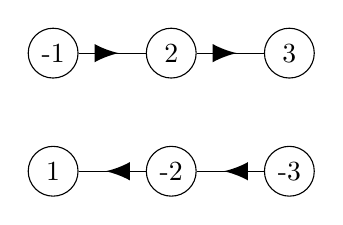
\begin{tikzpicture}[x=1.5cm, y=1.5cm
    ,every edge/.style={
        draw,
        postaction={decorate,
                    decoration={markings,mark=at position .6 with
		    {\arrow[line width=2pt,black]{latex}}} } }
]
\vertex (a) at (0,0) {1};
\vertex (b) at (1,0) {-2};
\vertex (c) at (2,0) {-3};
\vertex (d) at (0,1) {-1};
\vertex (e) at (1,1) {2};
\vertex (f) at (2,1) {3};
\path
(b) edge (a) 
(c) edge (b)
(d) edge (e) 
(e) edge (f)
;
\end{tikzpicture}\]
\vfill

\[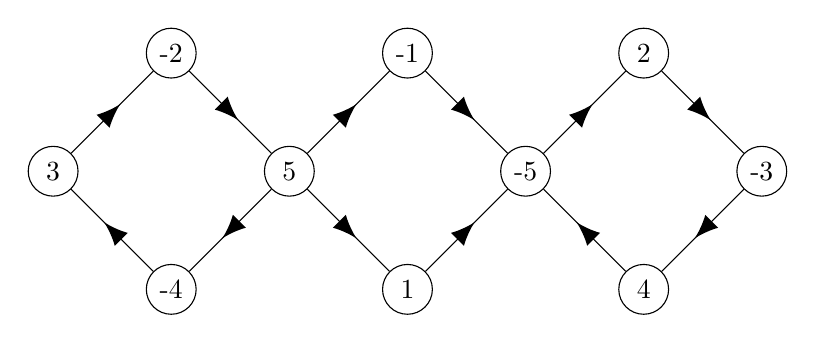
\begin{tikzpicture}[x=1.5cm, y=1.5cm
    ,every edge/.style={
        draw,
        postaction={decorate,
                    decoration={markings,mark=at position .6 with
		    {\arrow[line width=2pt,black]{latex}}} } }
]
\vertex (a) at (0,1) {3};
\vertex (b) at (1,2) {-2};
\vertex (c) at (1,0) {-4};
\vertex (d) at (2,1) {5};
\vertex (e) at (3,2) {-1};
\vertex (f) at (3,0) {1};
\vertex (g) at (4,1) {-5};
\vertex (h) at (5,2) {2};
\vertex (i) at (5,0) {4};
\vertex (j) at (6,1) {-3};
\path
(a) edge (b) 
(b) edge (d)
(c) edge (a)
(d) edge (c) edge (e) edge (f)
(e) edge (g)
(f) edge (g)
(g) edge (h)
(h) edge (j)
(i) edge (g) 
(j) edge (i) 
;
\end{tikzpicture}\]
\vfill

\[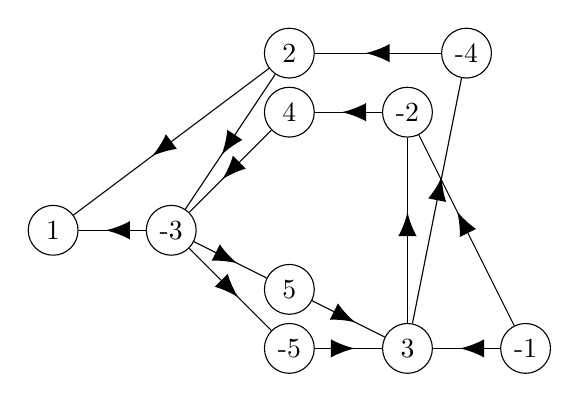
\begin{tikzpicture}[x=1.5cm, y=1.5cm
    ,every edge/.style={
        draw,
        postaction={decorate,
                    decoration={markings,mark=at position .6 with
		    {\arrow[line width=2pt,black]{latex}}} } }
]
\vertex (a) at (2,1) {-5};
\vertex (b) at (2,1.5) {5};
\vertex (c) at (3,1) {3};
\vertex (d) at (4,1) {-1};
\vertex (e) at (0,2) {1};
\vertex (f) at (1,2) {-3};
\vertex (g) at (2,3) {4};
\vertex (h) at (3,3) {-2};
\vertex (i) at (3.5,3.5) {-4};
\vertex (j) at (2,3.5) {2};
\path
(a) edge (c) 
(b) edge (c)
(c) edge (h) edge (i)
(d) edge (c) edge (h) 
(f) edge (a) edge (b) edge (e)
(g) edge (f)
(h) edge (g)
(i) edge (j)
(j) edge (e) edge (f)
;
\end{tikzpicture}\]
}
\end{document}
